\section{When a shared register should split}
\label{sec:yba-setup}

The opening problem needs a cost ledger before it needs an algorithm. Let \(q\in\mathbb R^2\) be a shared register, and let \(a,b\in\mathbb R^2\) be unit target vectors separated by angle \(\theta\in[0,\pi]\). Write
\begin{align}
 d^2&=\|a-b\|^2=2(1-\cos\theta),\nonumber\\
 \ell_1(q)&=\frac12\|q-a\|^2,\qquad
 \ell_2(q)=\frac12\|q-b\|^2 .
 \label{eq:num-toy-evaluator-losses}
\end{align}
The tasks supply distinct demands on one physical state. An authority weight \(\alpha\in[0,1]\) assigns task 1 a share \(\alpha\) and task 2 a share \(1-\alpha\). The weight is not an additional register in which both targets can be stored independently.

We choose the dimensionless static ledger
\begin{align}
 J(q,\alpha)={}&\alpha\ell_1(q)+(1-\alpha)\ell_2(q)
       +\gamma\alpha(1-\alpha)d^2 \nonumber\\
 &+\eta\big[(\alpha-\tfrac12)^2+
                  (1-\alpha-\tfrac12)^2\big],
 \qquad \gamma,\eta\geq0 .
 \label{eq:num-toy-conflict}
\end{align}
The first terms score the tasks. The term proportional to \(\gamma\) charges simultaneous incompatible use. The term proportional to \(\eta\) makes withdrawing authority from either task costly. These are declared modelling choices. Geometry alone does not force this particular conflict penalty, and a different physical ledger can produce a different purchase boundary.

For fixed \(\alpha\), differentiation with respect to the register gives
\begin{equation}
 q^*(\alpha)=\alpha a+(1-\alpha)b .
 \label{eq:num-toy-agent-b-optimum}
\end{equation}
Substituting this state eliminates the routine register motion. The weighted task residual becomes \(\alpha(1-\alpha)d^2/2\). If
\(A=d^2(1/2+\gamma)\), the entire remaining decision is
\begin{equation}
 J_{\mathrm{red}}(\alpha)
 =\frac A4+(2\eta-A)(\alpha-\tfrac12)^2 .
 \label{eq:num-toy-reduced-loss}
\end{equation}
A change of representation has already done useful work. Instead of following two components of \(q\) while changing an authority weight, we can decide the optimal allocation from the sign of one coefficient.

When \(A<2\eta\), balance is the unique optimum. When \(A>2\eta\), the two endpoints are optimal and one task receives all authority. At \(A=2\eta\), every allocation ties. Hence the best shared-register cost is
\begin{equation}
 J_{\mathrm{shared}}^*=\min\!\left(\frac A4,\frac\eta2\right).
 \label{eq:shared-minimum}
\end{equation}
Endpoint allocation does not satisfy both tasks. It pays the fairness price in order to stop paying the increasing shared residual and conflict cost. The plateau is an allocation decision, not the disappearance of the neglected task.

Now admit a different operation. The learner may purchase separate registers \(q_1,q_2\), set them to \(a,b\), and maintain balanced authority. We assume that this option has zero task residual and zero shared conflict, at a declared total price \(C_{\mathrm{part}}\geq0\). This price includes whatever maintenance or switching expense is being compared over the chosen static horizon. It is not automatically the one-step price of adding memory in a dynamical system. The enabled option has value
\begin{equation}
 J_{\mathrm{enabled}}^*
 =\min\!\left(\frac A4,\frac\eta2,C_{\mathrm{part}}\right).
 \label{eq:num-toy-agent-c-optimum}
\end{equation}
The strict split region is \(C_{\mathrm{part}}<J_{\mathrm{shared}}^*\). Since \(A\leq4(1/2+\gamma)\), such a region exists somewhere on \([0,\pi]\) precisely when
\begin{equation}
 C_{\mathrm{part}}<\min\!\left(\frac\eta2,\frac12+\gamma\right).
 \label{eq:split-region}
\end{equation}

Figure~\ref{fig:num-toy-shared-register} evaluates this ledger at \(\gamma=1\), \(\eta=0.8\) and \(C_{\mathrm{part}}=0.25\). The first crossing occurs at \(\theta\simeq0.84106867\) radians, where \(A/4=0.25\). Shared arbitration itself reaches its endpoint regime only at \(\theta\simeq1.08527820\), where \(A=1.6\). Capacity is worth buying before abandoning one task becomes the preferred shared solution.

\begin{figure*}[t]
\centering
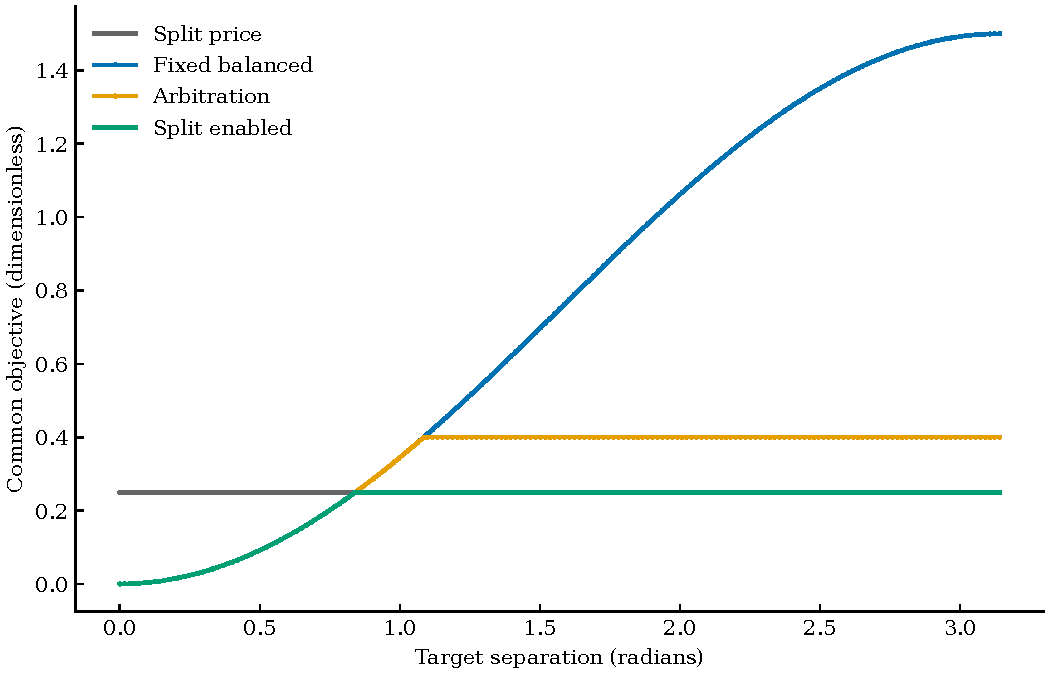
\includegraphics[width=0.82\textwidth]{figures/generated/slg-register-common-ledger-20261111.pdf}
\caption{When splitting the register pays. Static costs on the common ledger in Eq.~\eqref{eq:num-toy-conflict}, evaluated over 181 target separations. Fixed balance costs \(A/4\), optimised arbitration costs \(\min(A/4,0.4)\), and split-enabled allocation costs \(\min(A/4,0.4,0.25)\). All three curves coincide below \(0.8411\) radians, with the green result drawn on top. Above that crossing the green plateau is exactly the grey split-price reference, not a separate lower curve. Arbitration remains equal to fixed balance until \(1.0853\) radians and then caps at \(0.4\). The angle measures target separation. These are calculated static option boundaries, not measured dynamical or biological transitions.}
\label{fig:num-toy-shared-register}
\label{fig:slg-register-common-ledger-20261111}
\end{figure*}

The comparison would be misleading if fixed balance omitted a conflict charge that arbitration had to pay. Its cost here is \(A/4\), not merely the task residual \(d^2/8\). The policy classes are nested, so enabling allocation and then splitting cannot raise their optimised ledger values. The informative calculation is where the extra operation earns its price and which capacity assumption makes that possible.

The geometric interpretation also needs care. At the balanced optimum, the two nonzero task gradients are antiparallel for every \(d>0\). Varying \(\theta\) changes their magnitude, not a gradient angle that rotates continuously from agreement to opposition. In the general allocation optimum,
\(\nabla\ell_1=-(1-\alpha)(a-b)\) and
\(\nabla\ell_2=\alpha(a-b)\).
The register is a clean example of competing demands because those demands and the available operations are visible. To turn the static comparison into learning, we must now specify which state change a controller can actually buy.
